\section{Data Acquisition}
\label{sec:2_3_data_acquisition}
\begin{figure}[h!]
\centering
%left top right top
 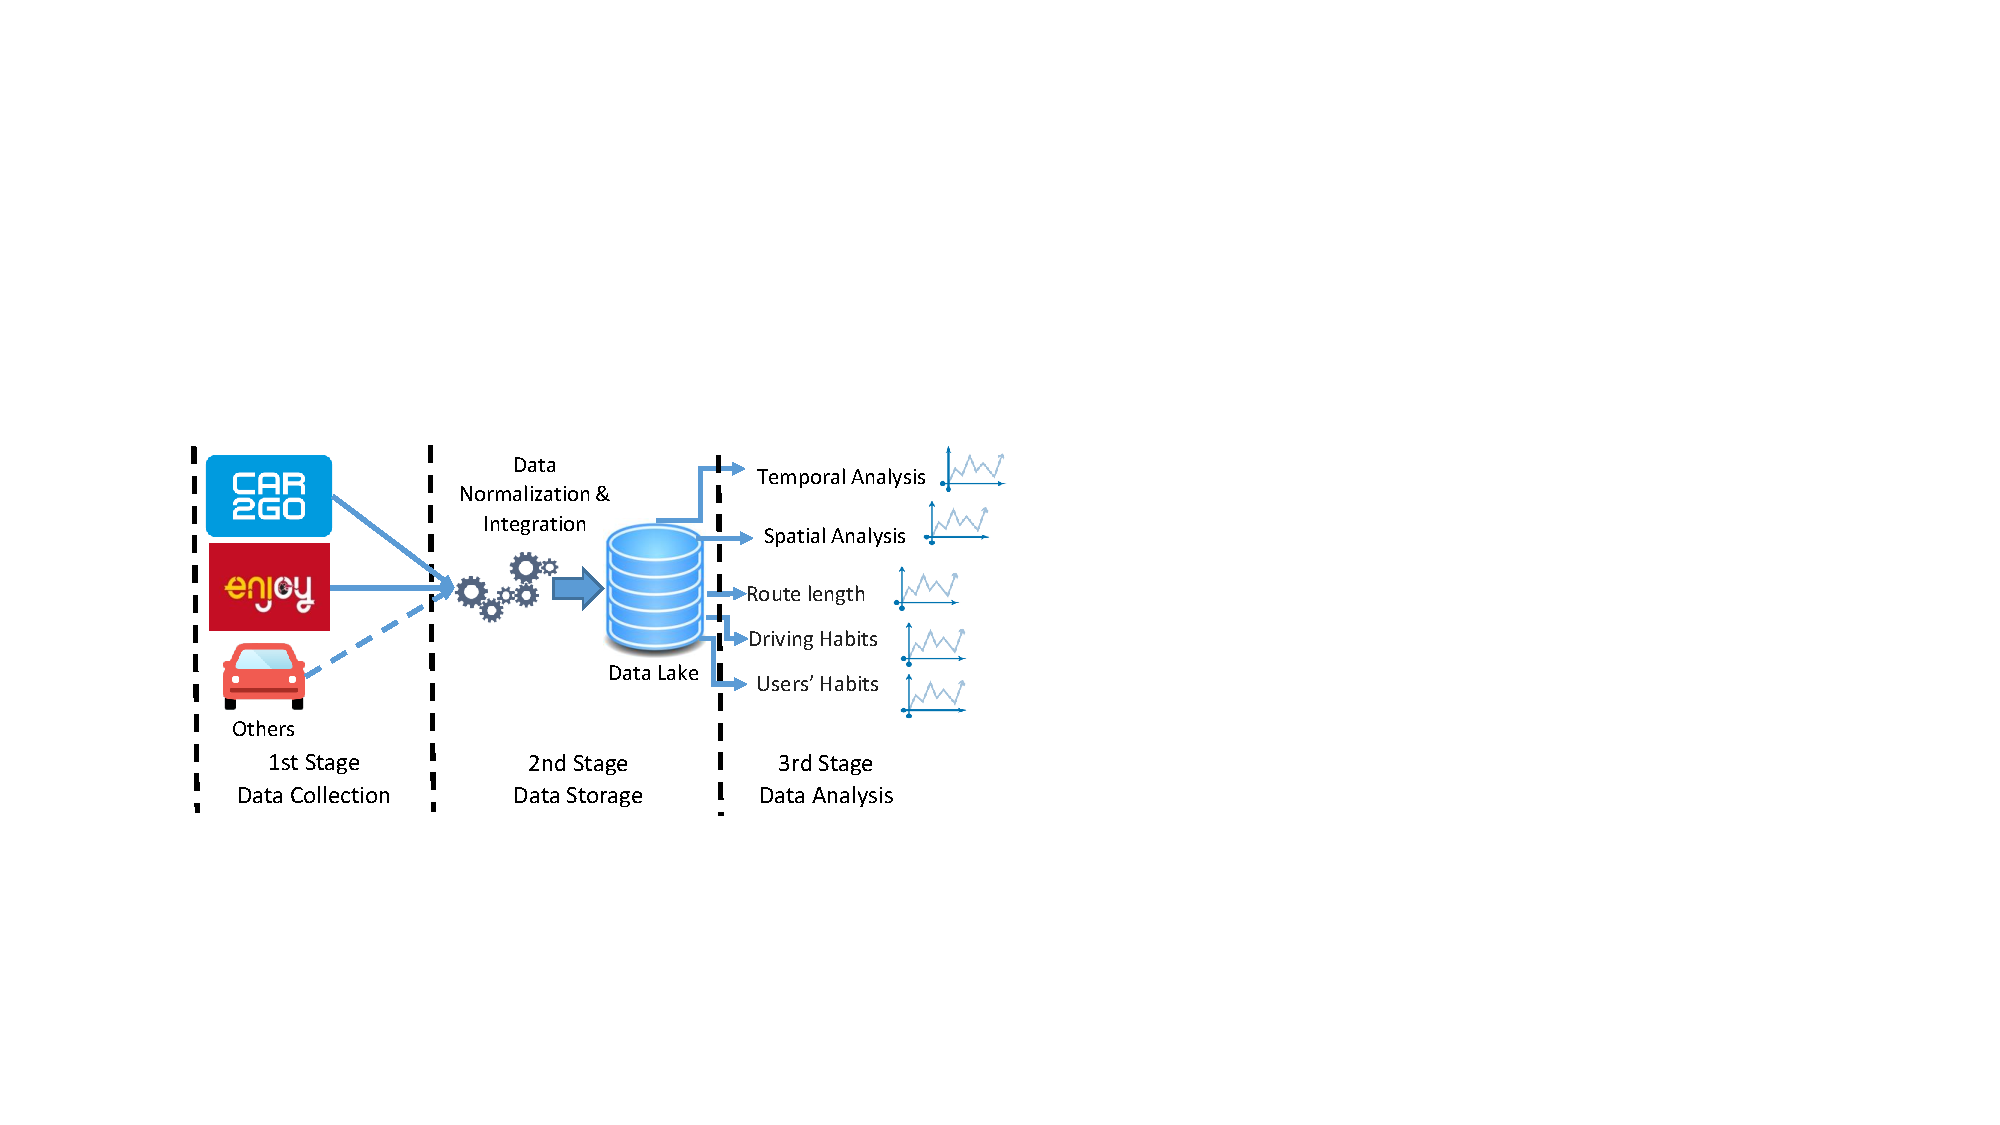
\includegraphics[trim=3cm 4.5cm 17cm 7.2cm,clip, width=0.95\columnwidth]{figures/framework_schema.pdf}
 \caption{\tool overview\label{fig:2_3_c2_framework}}
\end{figure}


In this section, I provide a description of \tool structure. Figure~\ref{fig:2_3_c2_framework} depicts the architecture of \tool, composed by a first module for the data acquisition, by a second module for data normalization and integration, and then a third  module for the data analysis.

The first module consists in the data acquisition from the car sharing platforms of interest. These typically expose information about cars' location when available for rental through a web-service approach. 

For this module I design two crawlers, one for the car2go and one for the Enjoy car sharing platforms. They retrieve, at each time instant, which cars are available in a given city.

While car2go offers public APIs~\cite{car2goAPI}, Enjoy does not provide to users such a service. For this reason I reverse engineer the Enjoy web portal. By leveraging the Chrome Developer Tools, I investigate the information exchanged with the Enjoy web portal while asking the list of available cars. Through this analysis, the software obtains both the URL used to request the list of available cars, and how fetch the data for a specific city.
Both system return the currently available cars using a JSON file.

Each time the system downloads a JSON, a \textit{snapshot} describing which cars are parked and ready for rental. Basically, the \textit{snapshot} is a list containing all cars and their attributes.

In a nutshell, a car is described by the car sharing web-service as an object annotated by several information, like plate, vehicle identification number (VIN), location, fuel level, model, etc. 
All the data represented in this object is useful for the customers e.g., to choose which car to rent.
This object is only present if the car is available, i.e., it is parked and free for a rental. Its state changes over time. In particular, a car disappears when a customer reserves and rents it, and then it reappears when the customer ends the rental (likely in a different location).


At each time $t$, the software gets the JSON snapshot $S$ listing the available cars. 
%We take a snapshot \textit{$S$} every minute to balance aggressiveness of the crawler, and time resolution. 
%At each time t, we obtain from each platform the JSON snapshot S detailing the available cars. 
The sampling period has been set to one minute, to balance aggressiveness of the crawler and a reasonable time resolution.
$S$ describes each available car with several fields, some of them being in common between the considered companies, but in general with different format.
For this study, I collect each car unique identifier and current geo-location indication.
These are obtained from the \textit{VIN} or \textit{plate} field, and the \textit{coordinates} field which describes the \textit{longitude} and the \textit{latitude} of the in-car GPS used to localize it when  parked.\footnote{The GPS coordinates are only available if a car is parked and available. There is no risk for users' privacy during rentals. In addition no user's identifier is exposed. Therefore data is totally anonymized as there is no means to know who booked a car.}
In addition to these fields, the car sharing JSON description may provide other information, e.g., the \textit{street address} corresponding to the coordinates, the \textit{fuel} level, the \textit{car interior status} the \textit{engine type}, etc. Since each platform uses its own data and format, I design a data integration step to have common names for fields containing the same information, if present.

\section{Data Normalization and Integration}
\label{sec:2_4_data_normalization}
In this second module I illustrates hoe \tool processes and consolidate each snapshot to obtain \emph{parking} and \emph{bookings} periods for each car. A \emph{parking} is time where the car is available for a user ride. On the other hand a \emph{bookings} is time elapsing two parking where the car is not tracked by the system. The intuition is to track the availability of each car on the car sharing platform, and rebuild the historic parking and booking periods over time: when a customer books a car, the latter ``disappears'' from the system. The framework records this event, with the initial time and position of a new booking. When the customer ends the booking, the car ``reappears'' in the system. The software records this event, with the final time and position of the booking. For the same car, a new parking period starts.

Harvested data is unstructured, and may grow large. Thus I leverage on \textit{MongoDB}, a NoSQL document-based database. A MongoDB database includes a set collections, i.e., groups of documents. Each document is a set of key-value pairs, organized in a JSON structure. The schema-less structure of MongoDB fits well in this work, because it can handle in the same collection documents defined with different key-value pairs. I decide to rely on such a system as I can easily manage the different field structures of providers, car2go and Enjoy in this use case. In addition, MongoDB offers a great integration with Python through the \textit{pymongo} module.

Four different collections compose the MongoDB data lake:  \textit{ActiveBookings}, \textit{ActiveParkings}, \textit{PermanentBookings}, and \textit{PermanentParkings}. 
\textit{ActiveBookings} and \textit{ActiveParkings} are collections used to store information about the current status of cars (currently booked or parked respectively). These are temporary structures that make it easier to query each car last observed status, and update it. These are also instrumentals for a real-time analysis of the system, e.g., to count how many cars are currently booked or available.
\textit{PermanentBookings} and \textit{PermanentParkings} collections store the history of past state of cars, for past bookings and parkings, respectively.

For the documents in the bookings collections I augment information by inserting also the expected route driving time, and the public transportation duration on the same origin-destination pair. These two piece of information are obtained through the Google Directions API using the initial and the final coordinates as indication of the path.

The most important fields in the \textit{ActiveBookings}, and the \textit{PermanentBookings} collections are:
\begin{itemize}
\setlength\itemsep{0.1em}
\item \textit{CarID}: the unique identifier of the car;
\item \textit{InitTime}: the initial time of the booking;
\item \textit{FinalTime}:  the final time of the booking;
\item \textit{InitCoords}:  the GPS coordinates of the booking star location, i.e., where the users picked up the car;
\item \textit{FinalCoords}:  the GPS coordinates of the parking location where the car was dropped at the end of the booking;
\item \textit{DrivingTime}: The duration of the trip, expressed in seconds, as estimated by Google Directions API, following the best path;
\item \textit{PublicTransportTime}: The duration is expressed as arrival time of the best public transport trip, as estimated by Google Directions API, minus the \textit{InitTime};
\end{itemize}

Instead, the \textit{ActiveParkings} and the \textit{PermanentParkings} collections are characterized by the following fields:
\begin{itemize}
\setlength\itemsep{0.1em}
\item \textit{CarID}: the unique identifier of the car
\item \textit{InitTime}: the initial time of the parking
\item \textit{FinalTime}:  the final time of the parking
\item \textit{Coordinates}: the GPS coordinates of the parking spot 
\end{itemize}

\begin{figure}[t!]
 \removelatexerror
 \scriptsize
  \begin{algorithm}[H]
   	\caption{Data acquisition at time $t$}
	\SetKwInOut{Input}{Input}\SetKwInOut{Output}{Output}
	\Input{$t$ - Current timestamp}
	\Input{$S$ - Available Cars (crawling result)}
	\BlankLine

	$AP$ = $Read(ActiveParkings)$ // Get previous available cars
	
	%\tcc{disappearedCars is a temporary list used to check the cars that %were visible, and that disappeared in the current crawling. In the %beginning the set will be equal to all the active Parkings}
	%$disappearedCars$ = $activeParkings$ \;
	\For(){$car_j$ in $S$}
	{
		\If{($car_j$  in $AP$)}
		{
			%\tcc{Update the parking information for that car with the %current timestamp}
			%$histogramNeighbours[final_time]$ = $current_timestamp$\;
			del $AP[car_j]$\;
		}
		\Else
		{
			$ActiveParkings.add(new~Parking(car_j,t))$\;		
			\If{($car_j$  in $ActiveBookings$)}
			{
				$FinalCoords = car_j[coords];$
				
				$ActiveBooking[car_j][FinalTime] = t$\;
				
				$InitCoords = ActiveBookings[car_j][InitCoords];$	
						
				\If{(checkCarMovement($InitCoords$,$FinalCoords$))}
				{
					$ActiveBooking[car_j][driving\_time]$ = $GoogleApi(driving,InitCoords,FinalCoords)$\;
					$ActiveBooking[car_j][PublicTranportTime]$ = $GoogleApi(public,InitCoords,FinalCoords)$\;
				}
				$MoveRow(car_j,ActiveBooking,PermanentBooking)$;
			}
			}
	}
	\For(){$car_j$ in $AP$}
	{
		$ActiveParking[car_j][FinalTime] = t$\;
		$MoveRow(car_j,ActiveParking,PermanentParking)$\;
		$ActiveBooking.add(new~Booking(car_j,t))$\;		
	}
  \end{algorithm}
   \caption{Pseudocode of the data acquisition algorithm}\label{pseudocodeCarInfoUpdate}
\end{figure}




I implemented an algorithm to extract booking and parking periods from snapshots, whose workflow is described in the pseudocode in Figure.~\ref{fig:3_2_c2_pseudocodeCarInfoUpdate}. Here I describe each  step.

I consider as inputs the snapshot $S$ and the current timestamp $t$.
Then I create a copy in the list $AP$ of parked cars observed in the previous snapshot (as stored in the $ActiveParkings$ collection) -- line 1. I need the $AP$ list to detect the cars that disappeared, i.e., have been booked at time $t$. This will be back explained later.

For each car $car_j$ in the current snapshot $S$, I check if the car is present in the $AP$ list. 
If so, it means that it did not change its status, i.e., it is still parked. Therefore, the car is removed from the $AP$ list, and nothing is changed -- lines 3-4.
Otherwise, either the car has been parked in this snapshot and the previous booking has finished, or the car is a new car added to the fleet. In both cases a new parking starts and I create a new document in the $ActiveParkings$ collection -- line 7. The \textit{new Parkings} function creates a new document, sets the $InitTime$ and $Coordinates$ keys as current timestamp and car GPS coordinates.
%with the current timestamp and the car GPS coordinates.

I next check if $car_j$ is present in the $ActiveBookings$ collection. If so, the car was booked until the previous snapshot and now it is back available. I thus finalize the previous booking and update its statistics. In particular, the tool sets the $FinalCoords$ and $FinalTime$ fields using the current car $coordinates$ and timestamp -- line 9-10. Next, I check if this booking includes an actual rental by checking if the initial position and final position differ -- line 11-12. Recall indeed that customers may simply book a car but not finalize the rental. Specifically, Enjoy (car2go) offers a grace period of 15 (20) minutes during which no charge is applied for a booking.

In case of an actual rental, I fetch the best path by i) car and ii) public transport from the  $InitPosition$ to the $FinalPosition$ of the rental. I leverage the Google Directions API for this -- line 13-14.\footnote{\url{https://enterprise.google.com/intl/it/maps/products/mapsapi.html}}
It is important to take into account that, while querying the public transportation time, the Google Directions API returns two pieces of information: how long the public transport takes to go from the initial to the final position, and the estimated arrival time. It is fundamental to use this second information because  it includes the time the user spends to reach the bus stop and wait for the bus. This is crucial, e.g., at night, when the first public transport solution may be available only several hours later.

After having processed all cars in the current snapshot, I iterate over the remaining cars in the $AP$ list. Those are the ones that were present in the previous snapshot, but not in the current, i.e., the ones the new bookings. Finally, the software adds to the previous parking period by setting the $FinalTime$ in the $ActiveParking$ collection -- line 21-22. At last, the tool creates a new booking via the \textit{new Booking} function -- line 23.


\begin{table}
	\setlength{\tabcolsep}{2.3pt}
	\centering
	\caption{Overview of car2go's data}
	\begin{tabular}{lcccc}
		\hline
		City &  City Size [$km^2$]\footnote{} & Population \footnotemark[\value{footnote}] &  Avg. Fleat & Bookings\\ 
		\hline
		\hline
		Columbus			  & 17 & 892k & 187 & 186k \\
		Florence 	  			& 34 & 372k & 220 & 333k \\
		Denver 		  			 & 36 & 727k & 312 & 348k \\
		Austin 		   			  & 31 & 964k & 315 & 377k \\
		Frankfurt 			   & 40 & 701k & 242 & 505k \\
		Toronto 				 & 49 & 3120k & 400 & 536k \\
		Amsterdam 			& 38 & 854k & 314 & 573k \\
		Montreal 				& 49 & 1704k & 429 & 606k \\
		New York City 	   & 77 & 8522k & 500 & 739k \\
		Turin 					    & 47 & 874k & 396 & 868k \\
		Munich 					 & 61 & 1464k & 478 & 916k \\
		Washington DC 	  & 64 & 705k & 563 & 919k \\
		Stuttgart 				 & 59 & 632k & 486 & 1001k \\
		Seattle 				   & 92 & 744k & 710 & 1134k \\
		Calgary 				  & 47 & 1239k & 552 & 1176k \\
		Rome 					  & 65 & 2837k & 582 & 1240k \\
		Rheinland 			   & 82 & 1688k & 648 & 1421k \\
		Vienna 					  & 72 & 1915k & 688 & 1702k \\
		Madrid 					 & 42 & 3233k & 424 & 2092k \\
		Milan 					   & 77 & 1396k & 776 & 2223k \\
		Hamburg 			  & 82 & 1833k & 812 & 2561k \\
		Vancouver 			 & 78 & 631k & 977 & 2701k \\
		Berlin 					  & 125 & 3769k & 1009 & 3091k \\
		%\\ \hline
		\hline
		\label{tab:2_3_datasummary}
	\end{tabular}
\end{table}
\footnotetext{\url{wikipedia.org}}
I let \tool scrape car2go's data  \mc{prendere le date}. In total it is possible to count about 27 million bookings spread in 23 cities. The table \ref{tab:2_3_datasummary} reports a brief resume of all the bookings, parkings present in the data lake. 

\mc{devo prendere le date anche di enjoy}



\section{Data Analysis}
The third and final stage is the data analysis phase in which analytics modules query the MongoDB and obtain statistics. I rely on the Python programming language with Pandas and the GeoPandas libraries to deal with the data, the city zone definitions, provided by transport engineers as a shapefile, a popular geospatial vector data format, and the Geographical Information Systems (GIS) for the spatial analyses. I choose Python as it offer a large number of  libraries that easily interact with the different technologies like GIS, maps and MongoDB. In particular the usage of GeoPandas allow me to easily perform geographic analysis and split the city in many areas (or zones) of any possible shapes. I present more detailed characterization in chapter \ref{chap:3_charact}.


\section{Conclusion}
In this chapter I described the software pipeline, named \tool I used to harvest and store data from real FFCS providers. 

The first stage explains the data structures and how I snapshots the system getting all the car ready for a ride. 

The seconds step illustrates the algorithm that compares consecutive snapshots detecting car status variation. Here I introduced the two fundamental car status I use to describe each car history: \textit{parkings} and \textit{bookings}. 

The third briefly opens several scenarios on the analyses of this data.


